%%--------- Comandos especiales
\newcommand{\vecr}{\mathbf{r}}
\newcommand{\veck}{\mathbf{k}}
\newcommand{\nnet}{N_{\theta}(\mathbf{r})}
%%
\chapter{Solución a la ecuación de Ornstein-Zernike usando redes neuronales} % Main chapter title

\label{Cap3} % Change X to a consecutive number; for referencing this chapter elsewhere, use \ref{ChapterX}

%----------------------------------------------------------------------------------------
%	SECTION 1
%----------------------------------------------------------------------------------------

Las \emph{redes neuronales} fungen como aproximadores universales~\cite{hornikMultilayerFeedforwardNetworks1989, hornikApproximationCapabilitiesMultilayer1991, cybenkoApproximationSuperpositionsSigmoidal1989},
y como tal pueden ser utilizadas para aproximar cualquier función continua para un determinado tipo de arquitectura.
En particular, se espera que una red neuronal pueda servir como paramatrización de la
función puente en la condición de cerradura de la ecuación de OZ, y así evitar escoger
una aproximación en especial, y dejar que la red neuronal tome la forma necesaria
para resolver la ecuación integral.

En este capítulo se detalla la metodología creada y los fundamentos matemáticos bajo los
cuales se puede hacer uso de redes neuronales para resolver la ecuación de OZ.
Se comparan estos resultados con los obtenidos con simulación por computadora.
En el apéndice se describe la solución general a la ecuación de OZ, mientras que
en este capítulo se detalla su modificación para emplear redes neuronales.

\section{Parametrización de la función puente}

La ecuación de Ornstein-Zernike está dada por

\begin{subequations}
    \begin{align*}
         & c(\vecr) = h(\vecr) +
        n \int_{V}
        c(\vecr^{\prime})
        h(\lvert \vecr - \vecr^{\prime} \rvert)
        d\vecr^{\prime} \label{eq:oz1} \\
         & c(\vecr)
        = \exp{\left[
                -  \beta u(\vecr)
                +  \gamma(\vecr)
                + B(\vecr)
                \right]} -
        \gamma(\vecr)
        - 1
    \end{align*}
\end{subequations}

con la notación ya conocida para esta ecuación.

Sea $\nnet$ una red neuronal con pesos $\theta$. Se propone que
$\nnet$ reemplace a la función puente $B(\vecr)$ en la ecuación
anterior tal que ahora se tiene la siguiente expresión para la cerradura

\begin{equation}
    c(\vecr) = \exp{\left[
            -  \beta u(\vecr)
            +  \gamma(\vecr)
            + \nnet
            \right]} -
    \gamma(\vecr)
    - 1 ,
    \label{eq:parametrizacion}
\end{equation}

y la ecuación de OZ queda de la misma forma.
Se pretende trabajar a partir de esta hipótesis donde la función puente
pueda tomar cualquier valor en particular que permita la solución de la
ecuación de OZ.

%----------------------------------------------------------------------------------------
%	SECTION 2
%----------------------------------------------------------------------------------------

\section{Esquema de entrenamiento}
Ahora que se tiene la parametrización, se debe desarrollar una forma para ajustar los
pesos de la red neuronal $\nnet$, y que al mismo tiempo permita la solución
de la ecuación de OZ.

\subsection{Función de costo}
Para crear un esquema de entrenamiento se requiere primero de una \textbf{función de costo}
que sea utilizada para generar información del ajuste necesario de los pesos $\theta$.
Tomando en cuenta que el esquema iterativo de Piccard crea una sucesión de funciones
estimadas $\{\gamma_1(\vecr), \gamma_2(\vecr), \dots, \gamma_n(\vecr)\}$, se propone que la función de costo
sea

\begin{equation}
    J(\theta) = \left[\gamma_{n}(\vecr; \theta) - \gamma_{n-1}(\vecr; \theta) \right]^2
    \label{eq:costo}
\end{equation}

donde $\gamma_{n}(\vecr; \theta)$ es la enésima función estimada de $\gamma(\vecr)$
mediante el método iterativo. La notación $\gamma(\vecr; \theta)$ indica que depende
implícitamente de los pesos de la red neuronal, como se puede ver en el ecuación~\eqref{eq:parametrizacion}.
Esto significa que si los pesos de $\nnet$ cambian, entonces la función $\gamma$ debe cambiar.
Sin embargo, esto no significa que $\gamma$ depende \emph{directamente} de los pesos.

\subsection{Problema de optimización}
Usando la función de costo~\eqref{eq:costo} ahora se puede plantear un problema de optimización
que permita el ajuste de los pesos de $\nnet$.

El problema de optimización en este caso es \emph{sin restricciones} y está
definido de la siguiente forma

\begin{equation}
    \begin{aligned}
         & \underset{\theta}{\text{min}}
         & & J(\theta)
    \end{aligned}
    \label{eq:optimizacion}
\end{equation}

Esto significa que buscamos los parámetros óptimos $\theta^*$ que minimicen la diferencia
entre las iteraciones calculadas de las funciones $\gamma(\vecr; \theta).$
Este problema de optimización se puede resolver de forma iterativa, al mismo tiempo que
se resuelve la ecuación de OZ.

\subsection{Actualización de pesos}
El método iterativo empleado está basado en la técnica de \emph{descenso de gradiente}
para actualizar los pesos de la red neuronal.
Esto significa que en general, una regla de actualización está dada por una expresión
semejante a la siguiente

\begin{equation}
    \theta_{n+1} = \theta_n - \eta \nabla_{\theta} J(\theta) .
    \label{eq:gradiente}
\end{equation}

donde $\eta$ se conoce como la \emph{razón de aprendizaje}, y es un parámetro que controla
el tamaño de paso del gradiente hacia la dirección de descenso.

% TODO: Cambiar el nombre del apéndice
Independientemente de la expresión de la actualización de los pesos, este cálculo
requiere de la información del gradiente de la función de costo respecto a los pesos,
$\nabla_{\theta} J(\theta)$.
Para este caso en particular, el cálculo detallado del gradiente se describe en el apéndice.
Una vez que se tiene esta información, lo que resta es construir un algoritmo que use
este esquema de entrenamiento y que resuelva la ecuación de OZ.

\subsection{Solución a la ecuación de Ornstein-Zernike con redes neuronales}
Con todos los elementos necesarios, se puede entonces definir el esquema general para
la solución a la ecuación de Ornstein-Zernike usando redes neuronales.

Para resolver la ecuación de OZ con la parametrización~\eqref{eq:parametrizacion} se tienen lo siguientes pasos:

\begin{enumerate}
    \item Dado el potencial de interación $u(\vecr)$, se emplea la ecuación~\eqref{eq:parametrizacion} para obtener el valor de $c(\vecr; \theta),$ la cual ahora depende implícitamente de los pesos de $\nnet$. En este paso también se requiere de un valor inicial para $\gamma_{n}(\vecr),$ el cual se inicializa de acuerdo a la metodología de Ng de cinco puntos, descrita en el apéndice. %% TODO: Cambiar el nombre del apéndice
    \item La función $c(\vecr; \theta)$ se transforma mediante la transformada de Fourier, para obtener $\hat{c}(\veck; \theta)$.
    \item Se transforma mediante la transformada de Fourier toda la ecuación de OZ, y se deja en términos de la función $\hat{\gamma}(\veck)$. Usando la información encontrada sobre la función $\hat{c}(\veck; \theta)$, se encuentra una nueva función $\hat{\gamma}_{n+1}(\veck; \theta)$.
    \item Luego, se antitransforma la función $\hat{\gamma}_{n+1}(\veck; \theta)$ para obtener la nueva estimación, $\gamma_{n+1}(\vecr; \theta)$.
    \item Usando ambas estimaciones $\gamma_{n}$ y $\gamma_{n+1}$, se evalúa la función de costo~\eqref{eq:costo} y se realiza el cálculo del gradiente, $\nabla_{\theta} J(\theta)$.
    \item Se actualizan los pesos usando la expresión~\eqref{eq:gradiente}, y se reinicia el proceso. En la siguiente iteración, la función inicial será ahora $\gamma_{n+1}$, para entonces obtener una nueva estimación $\gamma_{n+2}$, y así sucesivamente.
\end{enumerate}

\subsection{Convergencia del entrenamiento}
El procedimiento descrito anteriormente se repite de forma indefinida hasta lograr la 
convergencia, dada por la siguiente expresión

\begin{equation}
    {\lvert \gamma_{n+1} - \gamma_{n} \rvert}^2 \leq \epsilon
    \label{eq:tolerancia}
\end{equation}

donde $\lvert \cdot \rvert$ indica el valor absoluto, y $\epsilon \in [0, 1]$.
En particular, la tolerancia en todos los experimentos realizados fue de
$\epsilon = \num{1e-5}$.
En otras palabras, se exige a la red neuronal ajustar sus pesos hasta que las estimaciones
sucesivas de las funciones $\gamma$ sean muy semejantes entre sí.

%----------------------------------------------------------------------------------------
%	SECTION 3
%----------------------------------------------------------------------------------------
\section{Implementación}
En esta sección se detallan los aspectos importantes de la implementación del método
descrito en la sección anterior, como lo son la arquitectura de la red neuronal, el método
de optimización, y la elección de las funciones de activación, así como los parámetros
utilizados para resolver la ecuación de OZ.

\subsection{Elección de optimizador}
La regla general de actualización de pesos~\eqref{eq:gradiente} fue implementada para 
resolver el problema de optimización, sin embargo, problemas numéricos impedían la
convergencia del entrenamiento.

Para resolver este problema se optó por utilizar el método \emph{Adam}~\cite{kingmaAdamMethodStochastic2017},
el cual es un método de optimización adecuado para entrenamiento de redes neuronales,
sobre todo cuando el gradiente puede ser \emph{disperso}, i.e. que muchas de sus entradas
sean cero.
El método \emph{Adam} emplea diversas reglas para ajustar la dirección de descenso del
gradiente, así como los hiperparámetros asociados al método. En particular, este método
utiliza dos hiperparámetros, $\beta_1$, que controla el promedio móvil
del gradiente calculado; y $\beta_2$, que controla el cuadrado del gradiente. Ambas
cantidades son necesarias para la convergencia óptima del algoritmo.

Las ecuaciones que definen al método de optimización son las siguientes

\begin{align}
    m &= \beta_1 m - (1 - \beta_1) \nabla_{\theta} J(\theta) \nonumber \\
    s &= \beta_2 s + (1 - \beta_2) \nabla_{\theta} J(\theta) \odot \nabla_{\theta} J(\theta) \nonumber \\
    \hat{m} &= \frac{m}{1 - \beta_1^t} \nonumber \\
    \hat{s} &= \frac{s}{1 - \beta_2^t} \nonumber \\
    \theta &= \theta + \eta \hat{m} \oslash \sqrt{\hat{s} + \varepsilon}
    \label{eq:adam}
\end{align}

donde $\odot$ significa multiplicación entrada por entrada, o producto de Hadamard;
$\oslash$ significa división entrada por entrada, o división de Hadamard;
y $\varepsilon$ es un número de tolerancia que impide la división por cero.

En los resultados presentados en esta sección, se emplearon los hiperparámetros con sus
valores estándar, $\beta_1=\num{0.9}$ y $\beta_2=\num{0.999}$.Es importante notar que
este método de optimización utiliza sus propios mecanismos para controlar los gradientes,
así como estos hiperparámetros. El valor de la \emph{razón de aprendizaje}, $\eta$
en la ecuación~\eqref{eq:gradiente}, utilizado en todos los experimentos fue de
$\eta=\num{1e-4}$.

\subsection{Arquitectura de la red neuronal}

\begin{figure}[t]
    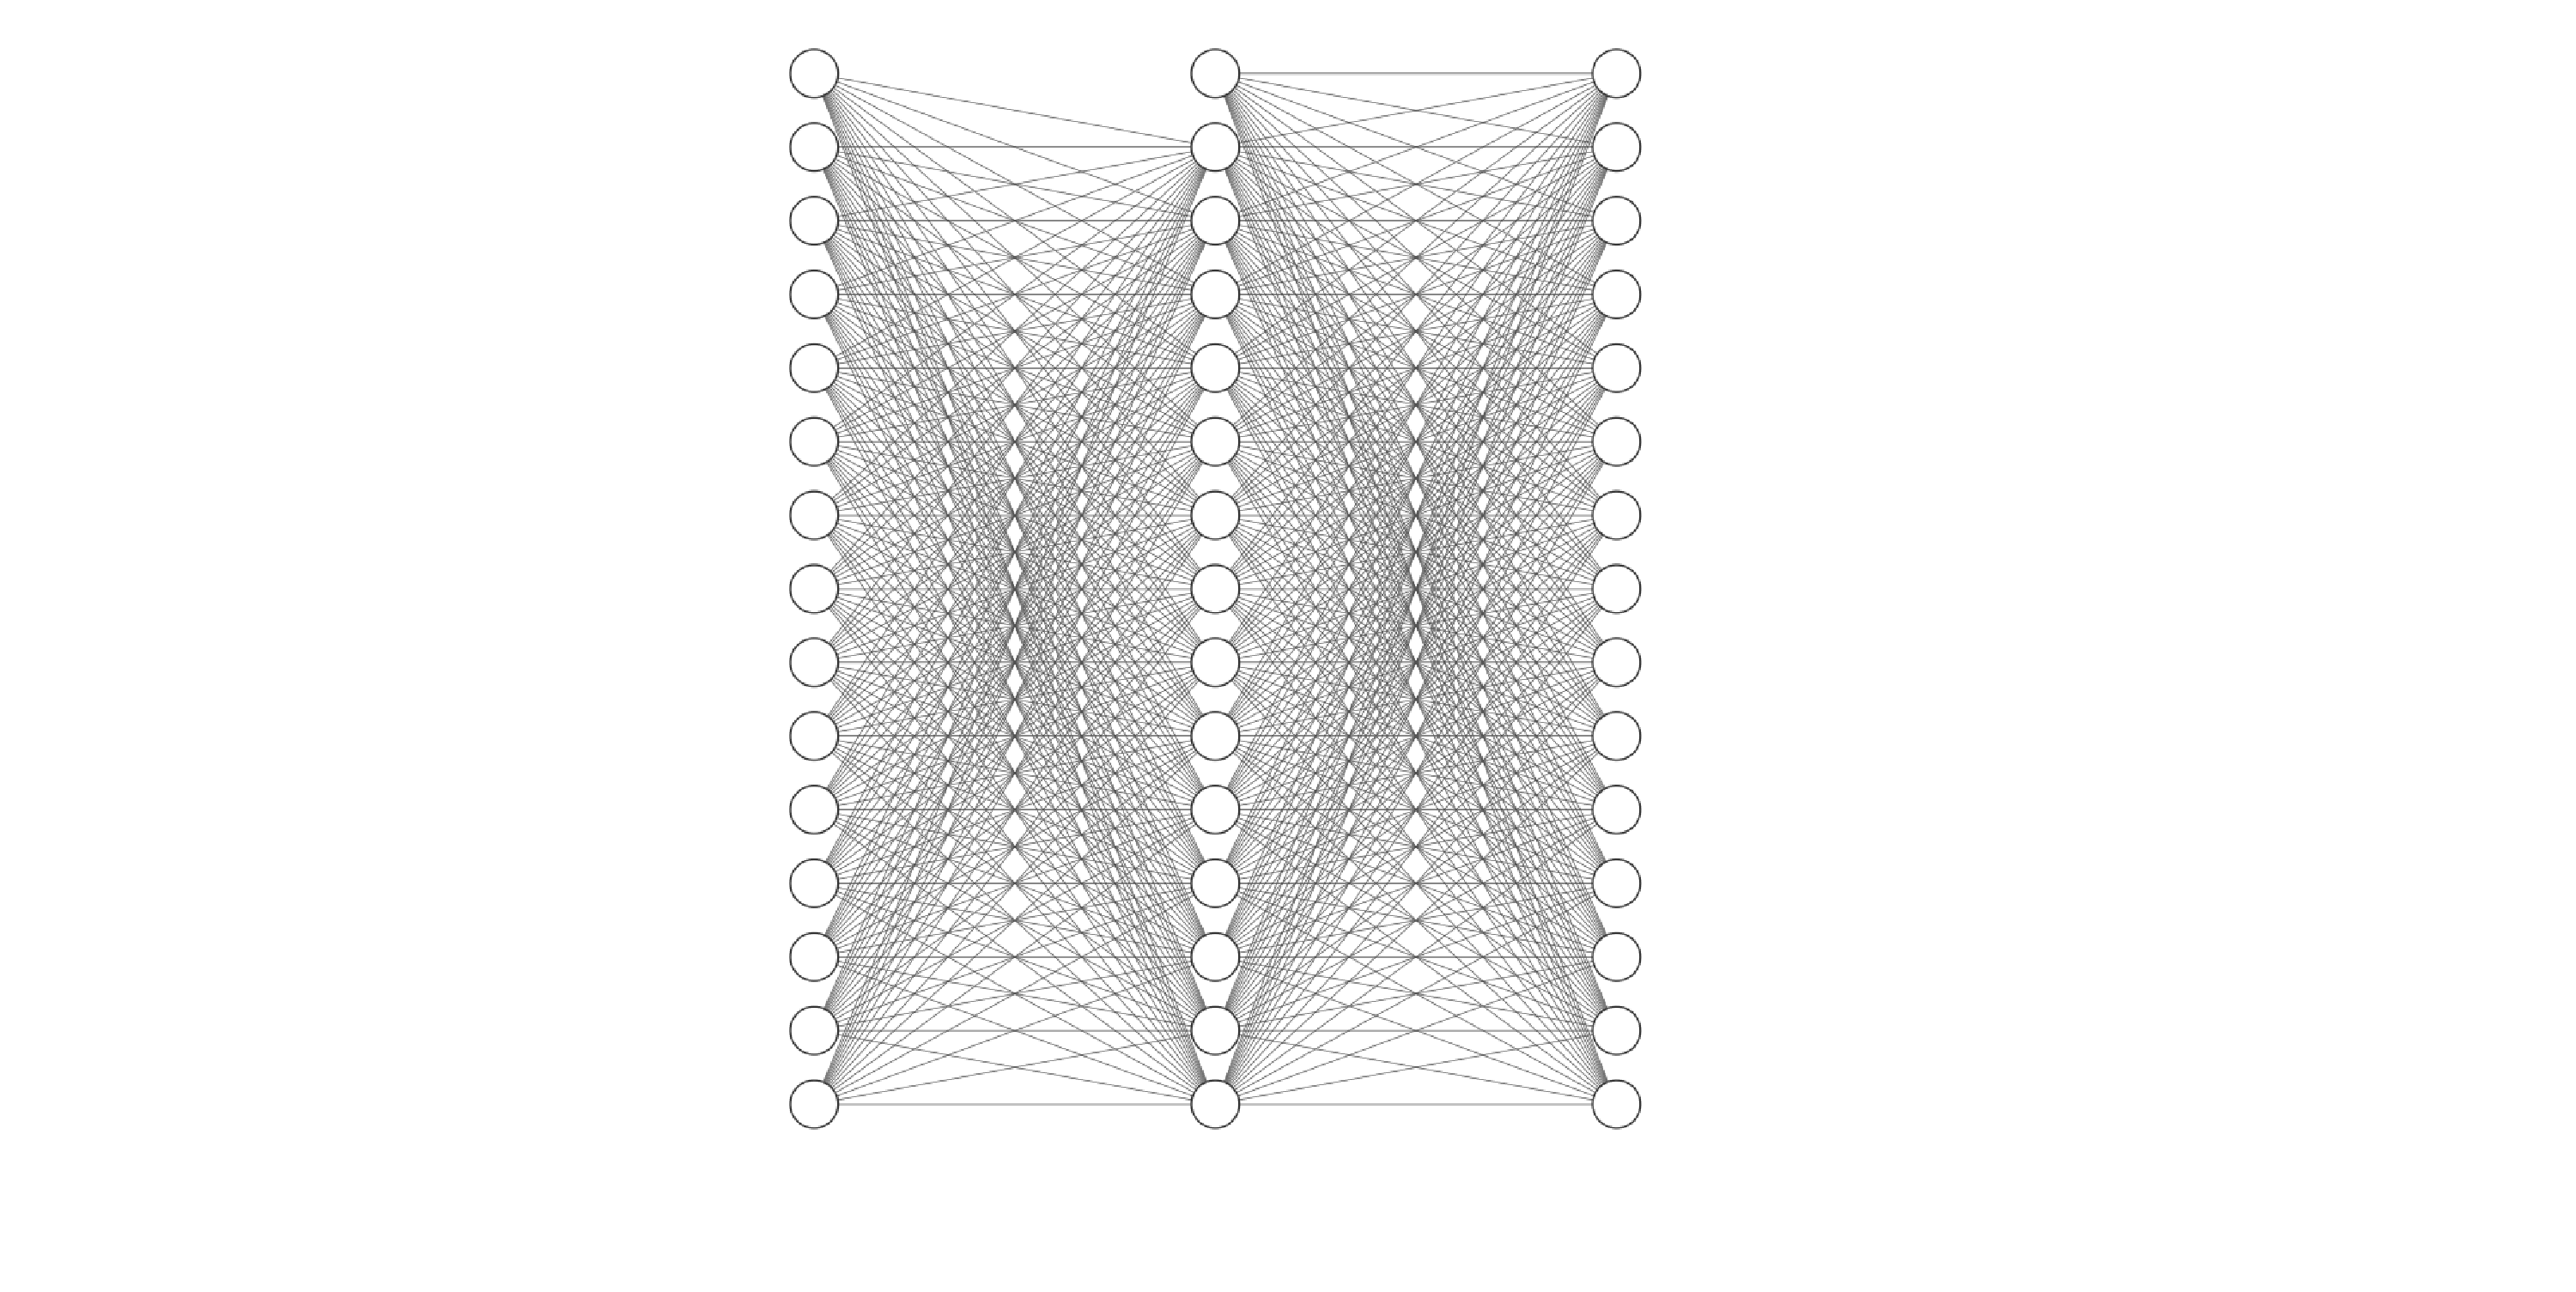
\includegraphics[width=\textwidth]{figuras/capitulo-3/neural-network.pdf}
    \vspace{-1.5cm}
    \caption{Esquema genérico de una red neuronal multicapa completamente conectada. Es importante notar la forma de la red, donde se tienen dos capas escondidas. Los círculos representan \emph{unidades} o \emph{nodos}, que están siendo evaluados por una función de activación. Los nodos que se ven separados de las capas (aquellos que están en la parte superior del esquema) son los \emph{sesgos} de las capas penúltima y última, respectivamente. La arquitectura usada en los resultados de este capítulo es diferente y más grande, pero tiene la misma estructura.}
    \label{fig:nn-esquema}
\end{figure}

La arquitectura de la red neuronal empleada en todos los experimentos es aquella que se
muestra en el esquema de la figura~\ref{fig:nn-esquema}, excepto por el número de unidades
en las capas ocultas.
Es decir, la arquitectura es de \emph{cuatro capas}, una capa de \emph{entrada} con una
unidad, dos capas ocultas con 1024 unidades cada una, y por último una capa de \emph{salida}
con una sola unidad.

La función de activación que se empleó fue la función \emph{ReLU}~\cite{glorotDeepSparseRectifier2011},
la cual está definida con la siguiente expresión

\begin{equation*}
    \text{ReLU}(x) = \text{max}{(0, x)} .
\end{equation*}

Esta función de activación se aplica a todas las capas a excepción de la capa de entrada.
Se escogió esta función de activación debido a que todas las más comunes ($\tanh, \text{softmax}$, etc.),
provocaban inconsistencias numéricas.

\subsection{Parámetros físicos}

% TODO: Poner la referencia a la ecuación del potencial
Para resolver la ecuación de OZ se empleó un radio de corte $r_c=7\sigma$, donde $\sigma$
es el diámetro de las partículas y tiene por valor $\sigma=1$.
El potencial empleado fue el de pseudo-esferas duras (Ref), tanto para la solución de la ecuación
de OZ como para los resultados obtenidos de simulación por computadora.

Se exploraron siete densidades diferentes en un rango de
$\phi \in [\num{0.15}, \num{0.45}]$, con $\Delta \phi = \num{0.05}$. Por cada valor
de la densidad se utilizó una partición de la densidad de 70 puntos para lograr la
convergencia del método iterativo cuando se resolvió la ecuación de OZ. En el caso de las
simulaciones por computadora, no se necesita esta partición.

%----------------------------------------------------------------------------------------
%	SECTION 4
%----------------------------------------------------------------------------------------
\section{Resultados}

\begin{figure}[p]
    \begin{tabular}{cc}
        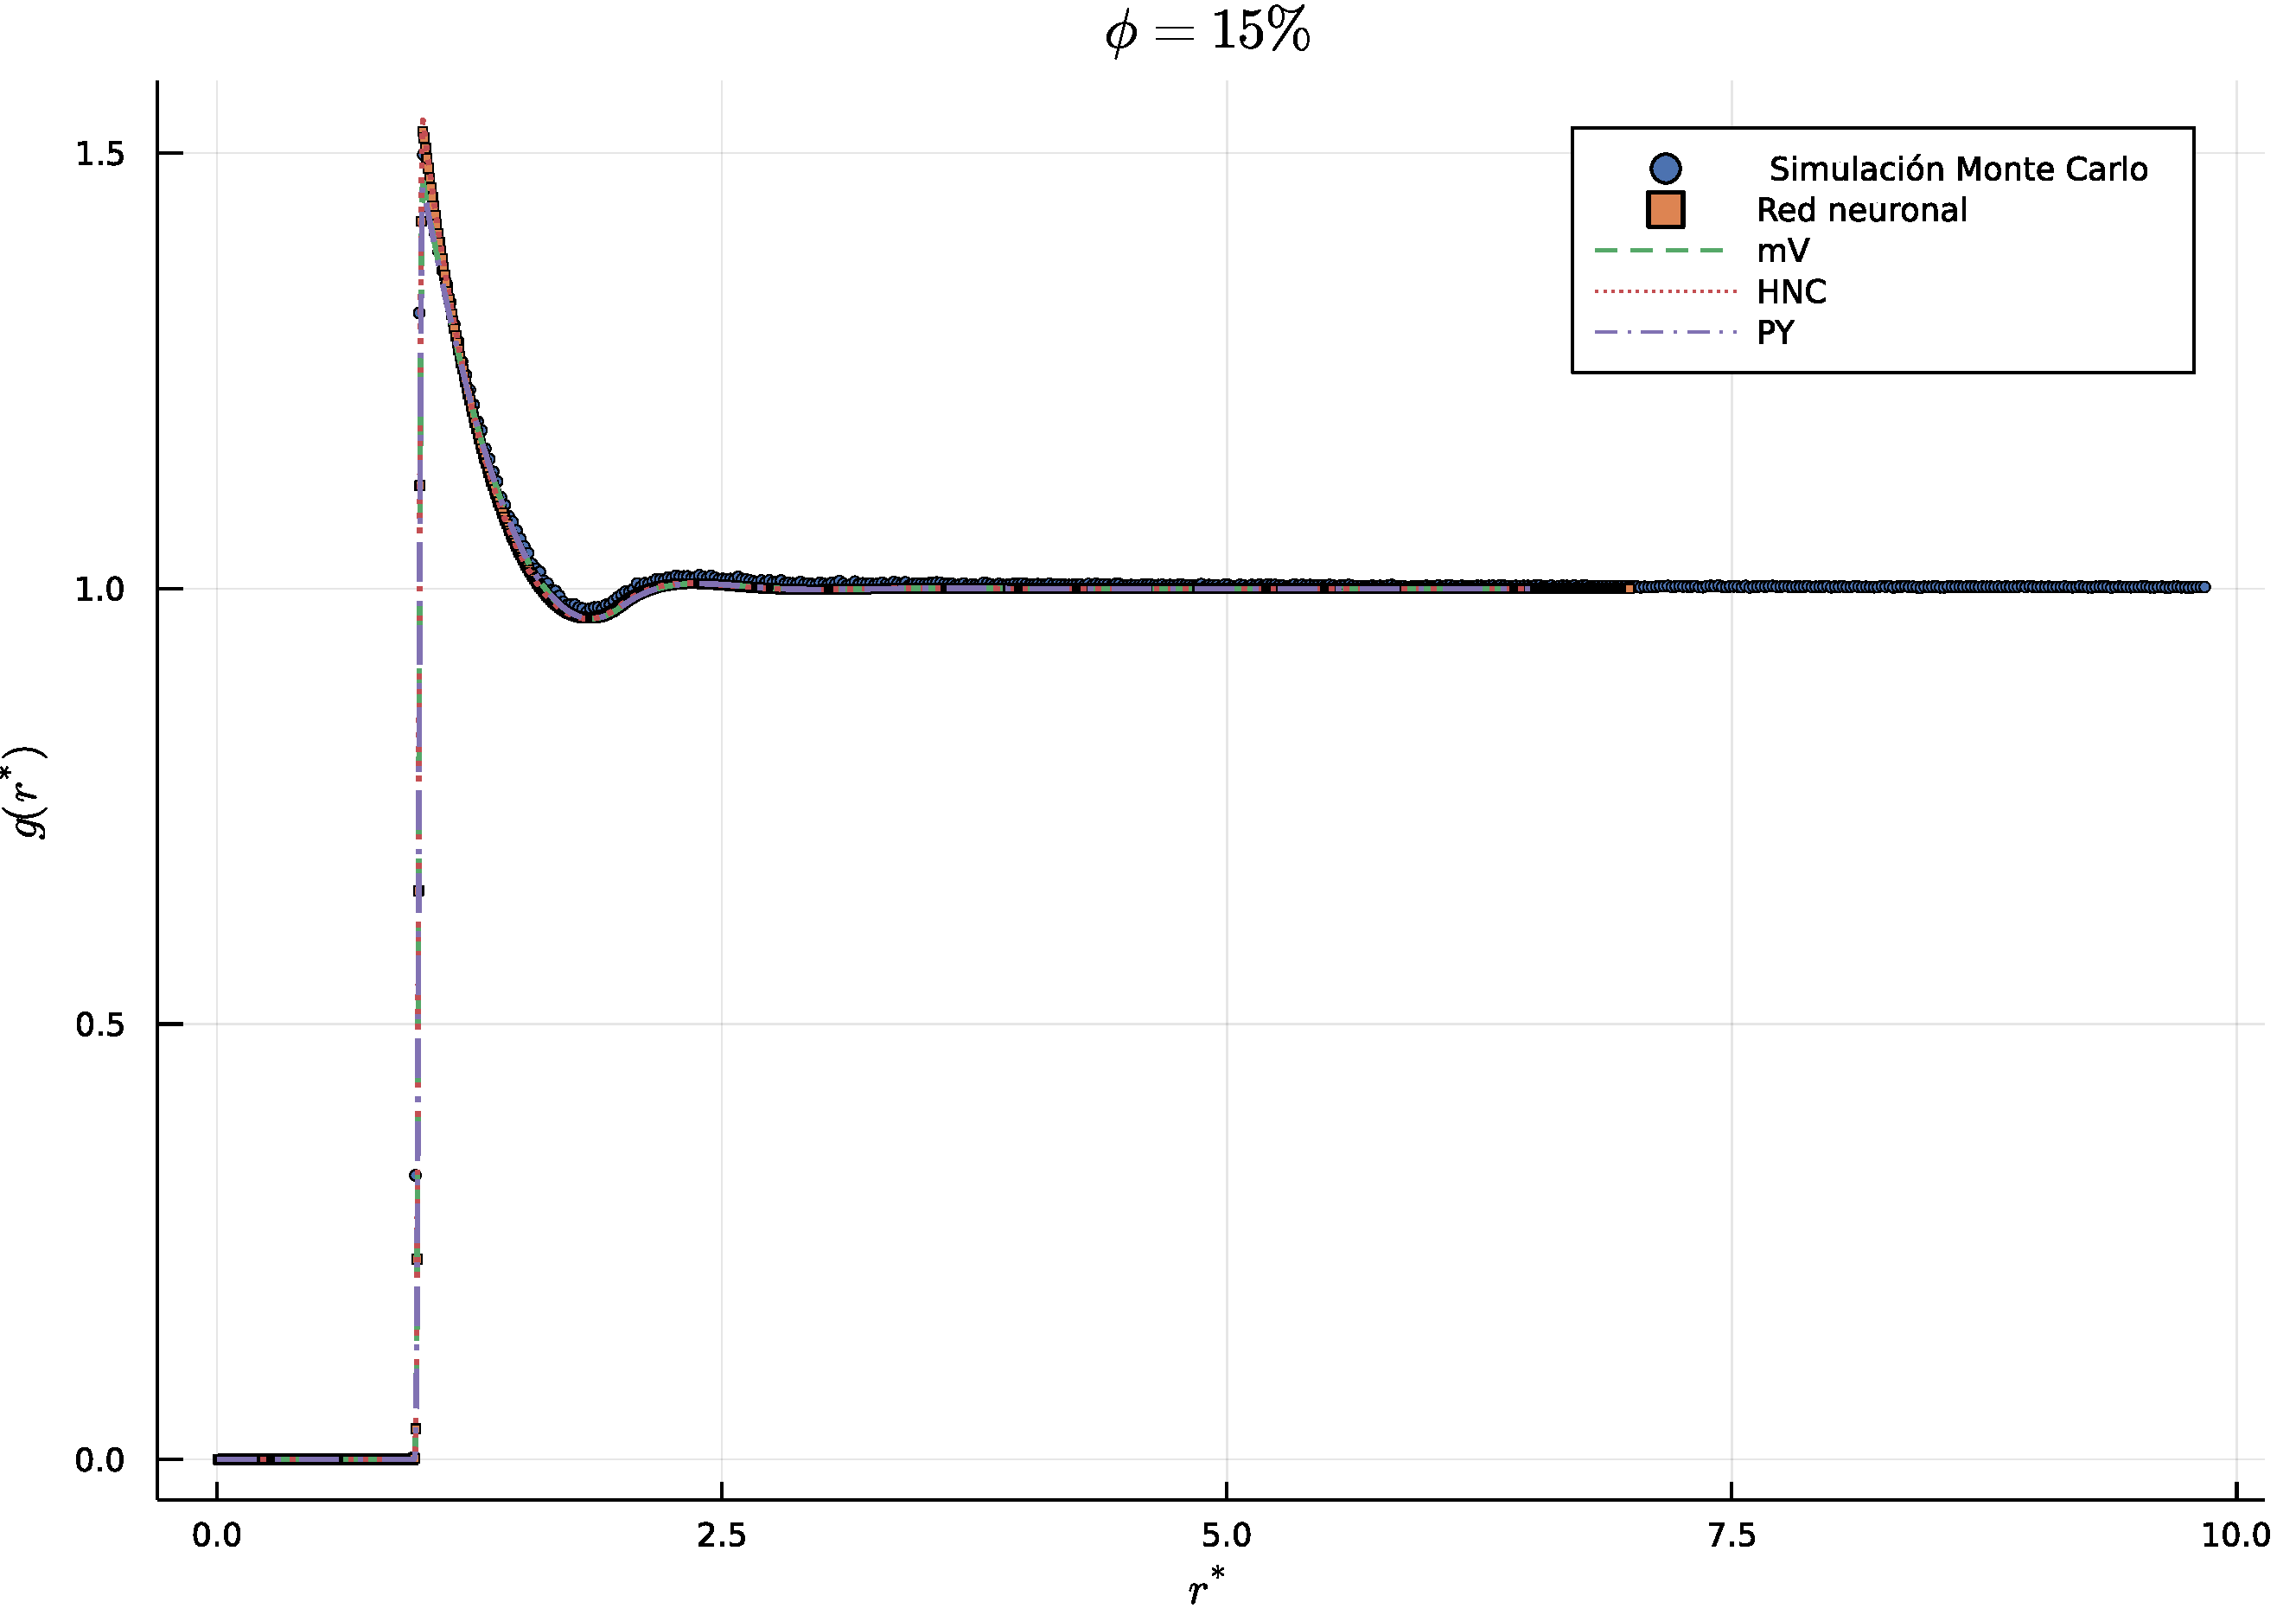
\includegraphics[width=0.47\textwidth]{figuras/capitulo-3/p=0.15.pdf} & 
        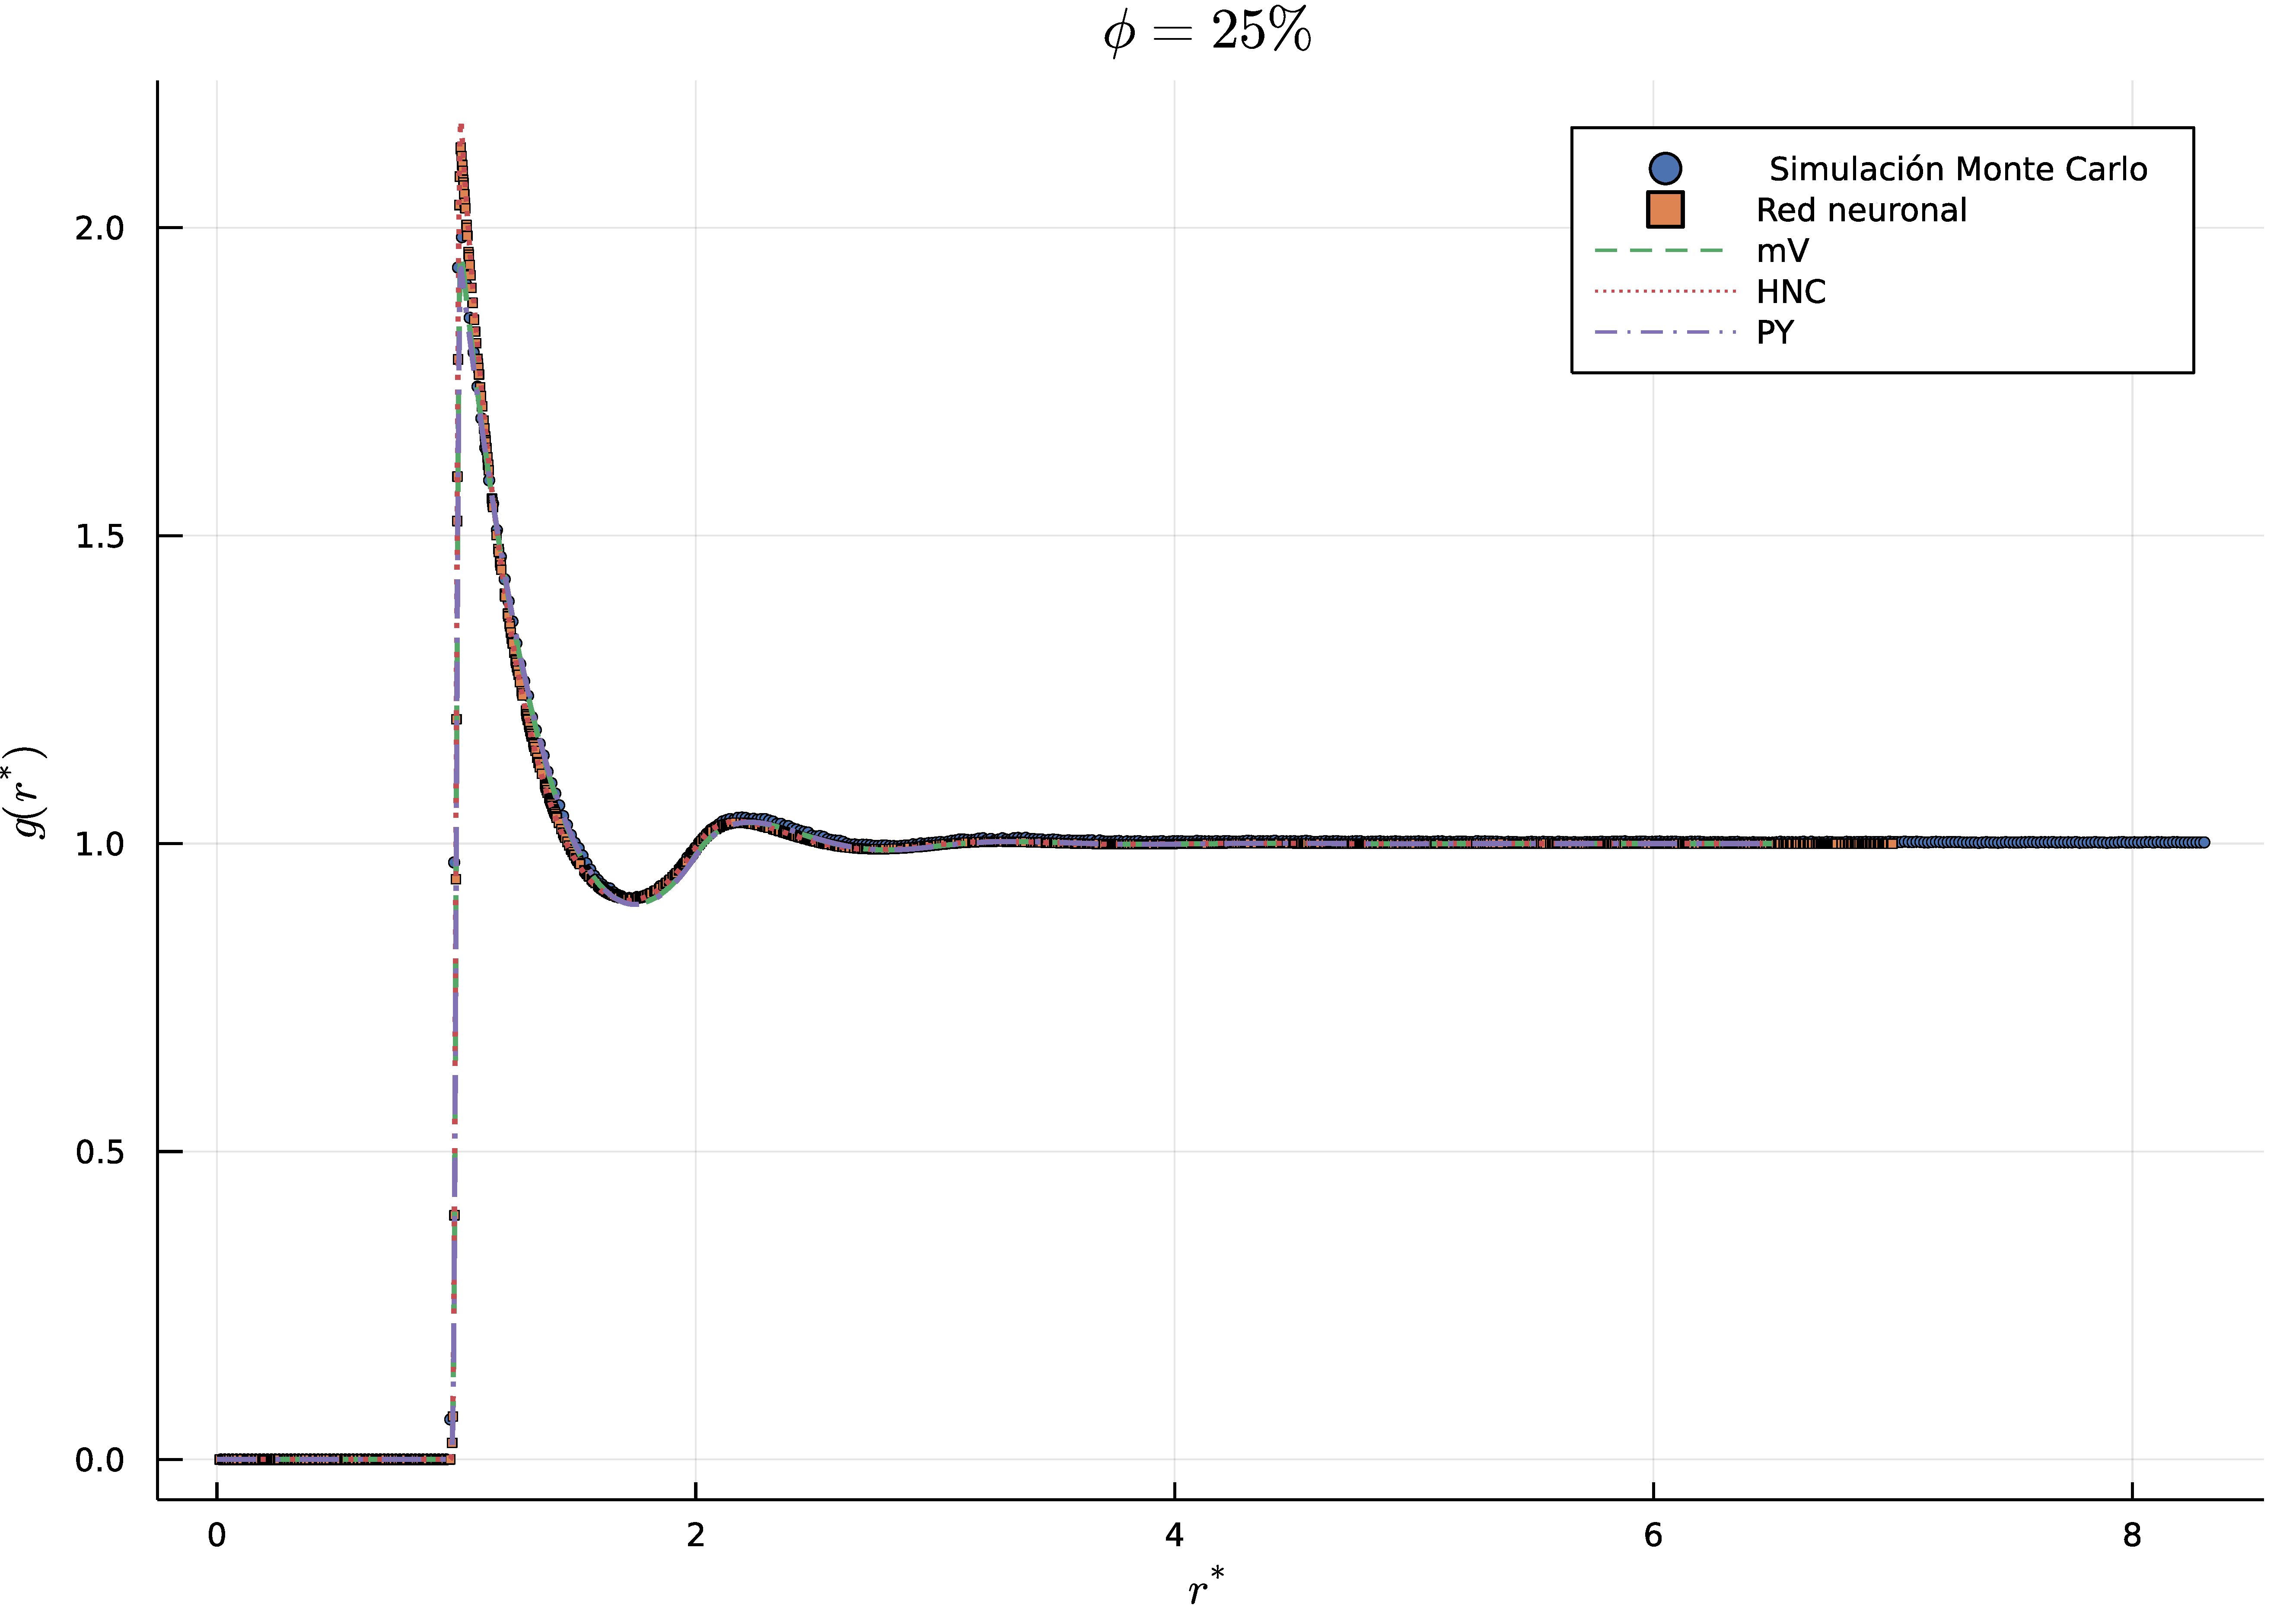
\includegraphics[width=0.47\textwidth]{figuras/capitulo-3/p=0.25.pdf} \\
        (a) & (b) \\[6pt]
        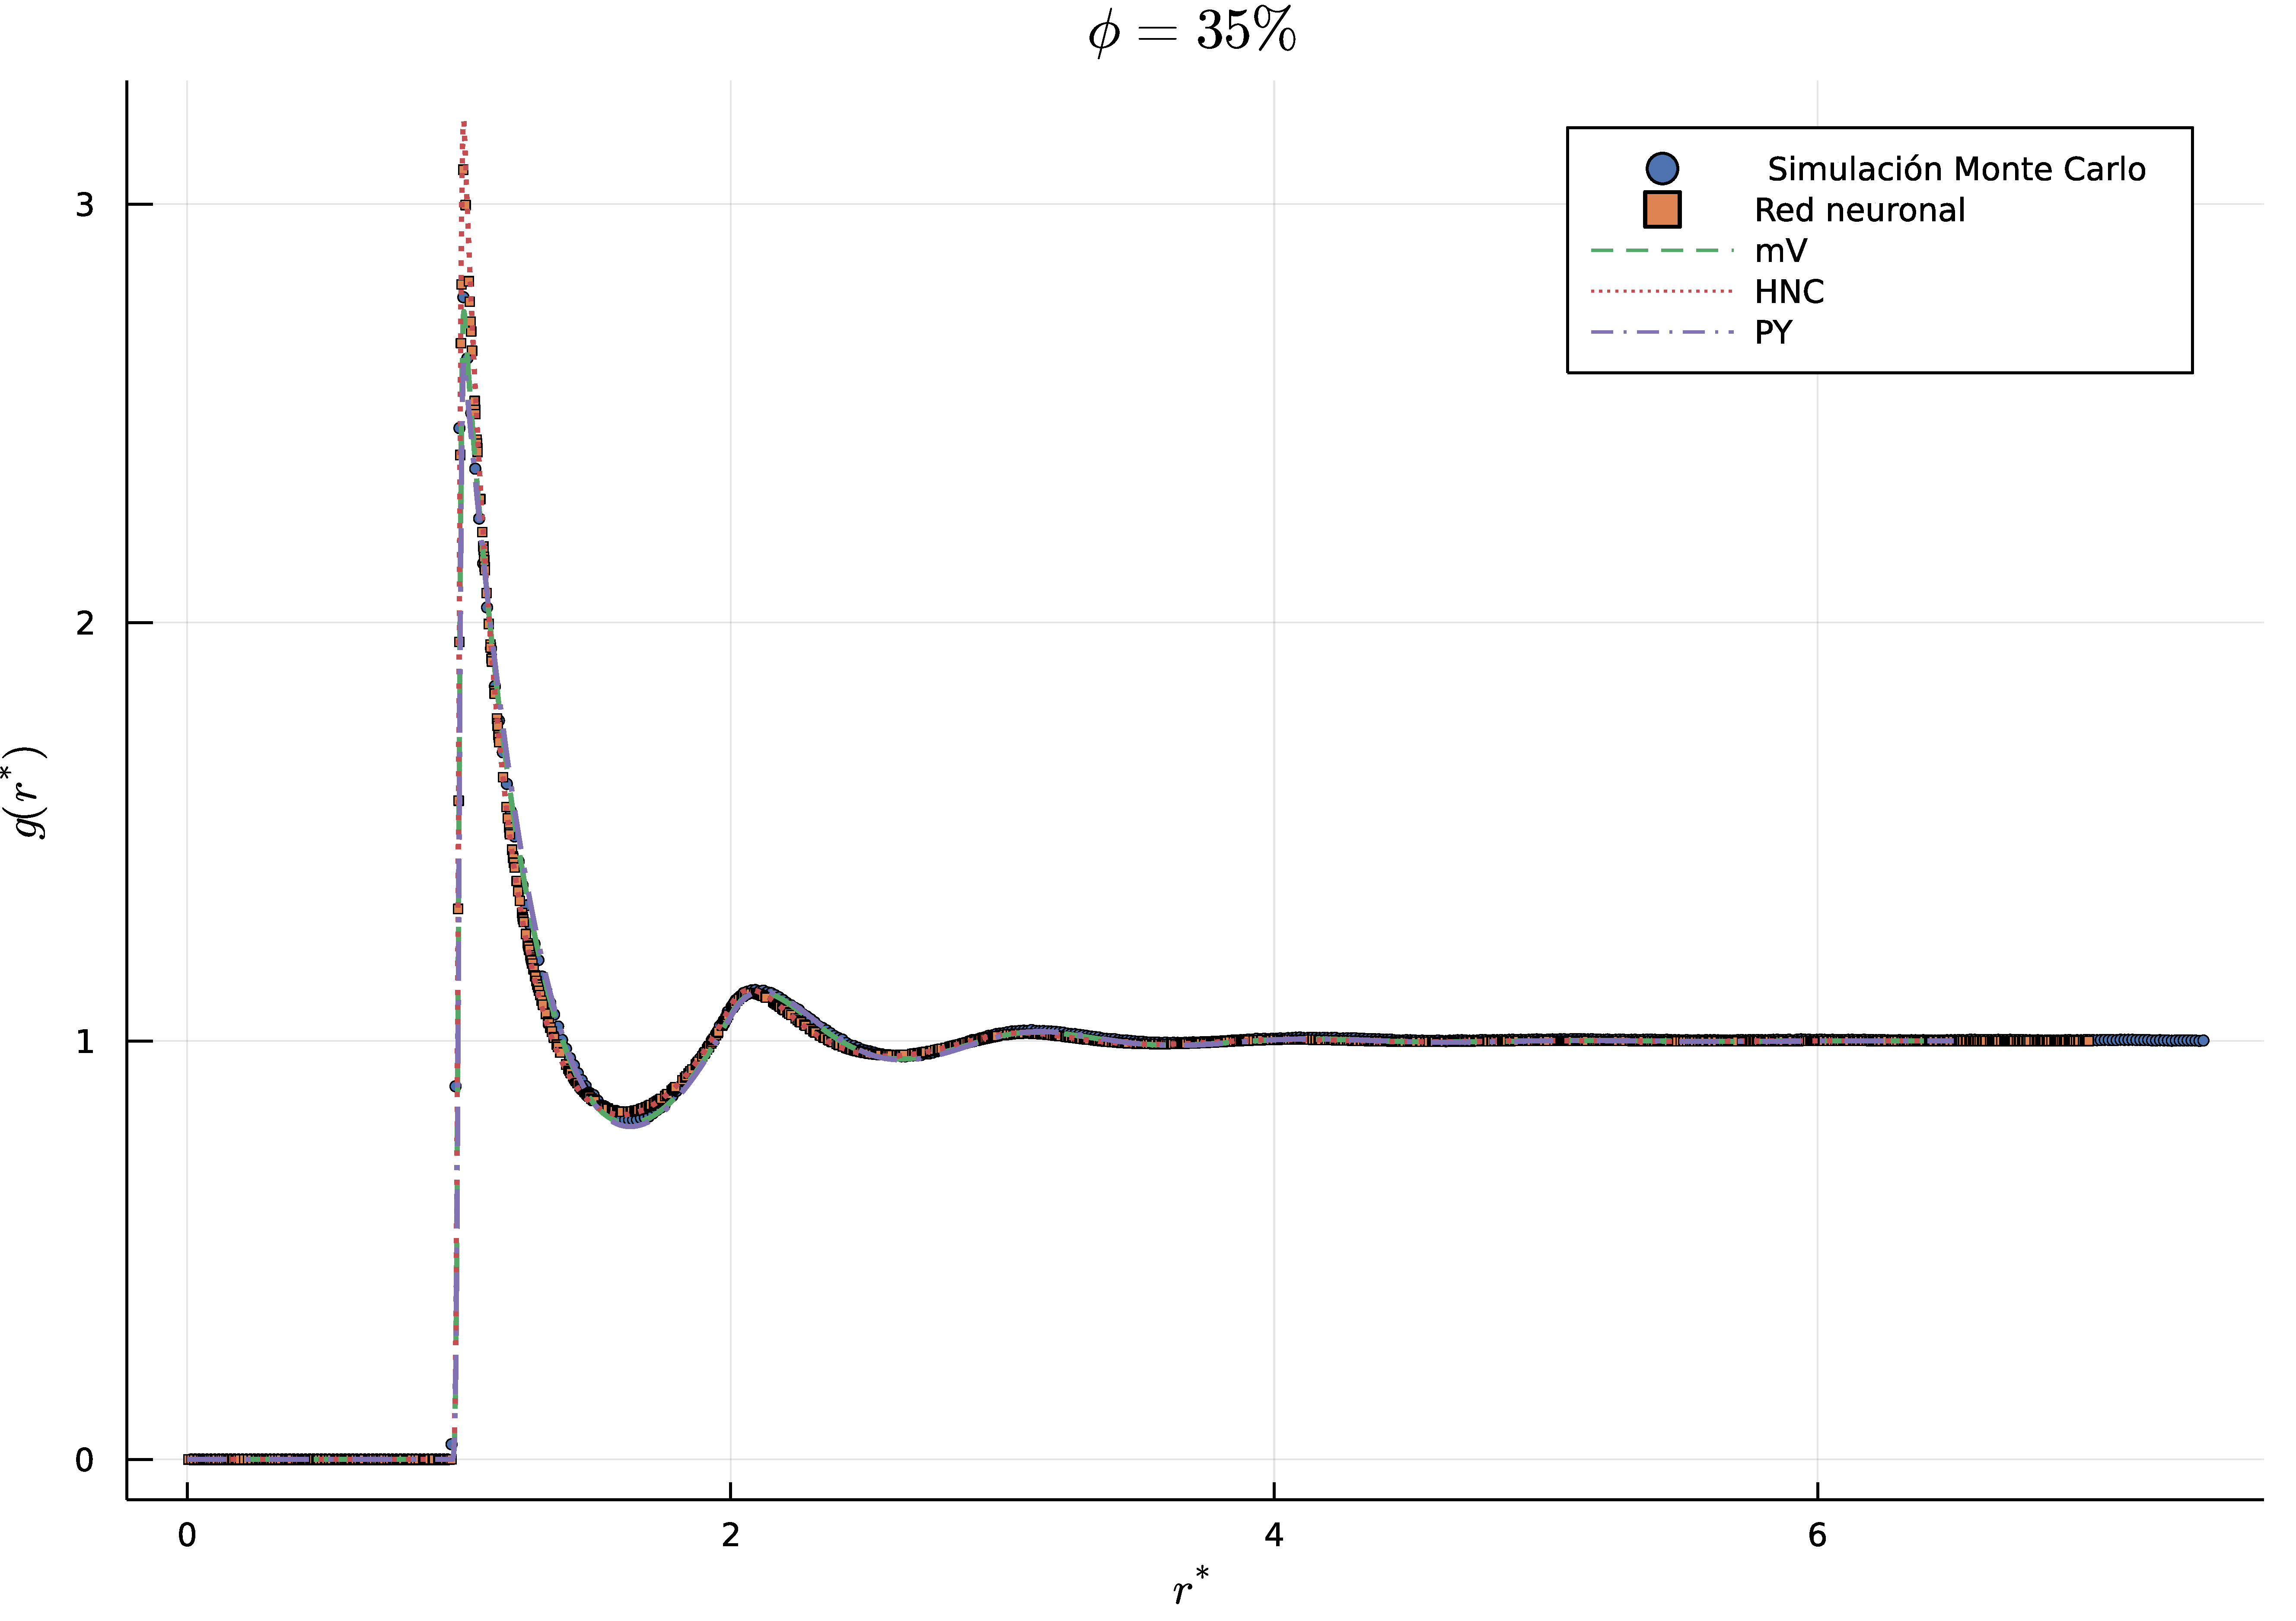
\includegraphics[width=0.47\textwidth]{figuras/capitulo-3/p=0.35.pdf} &   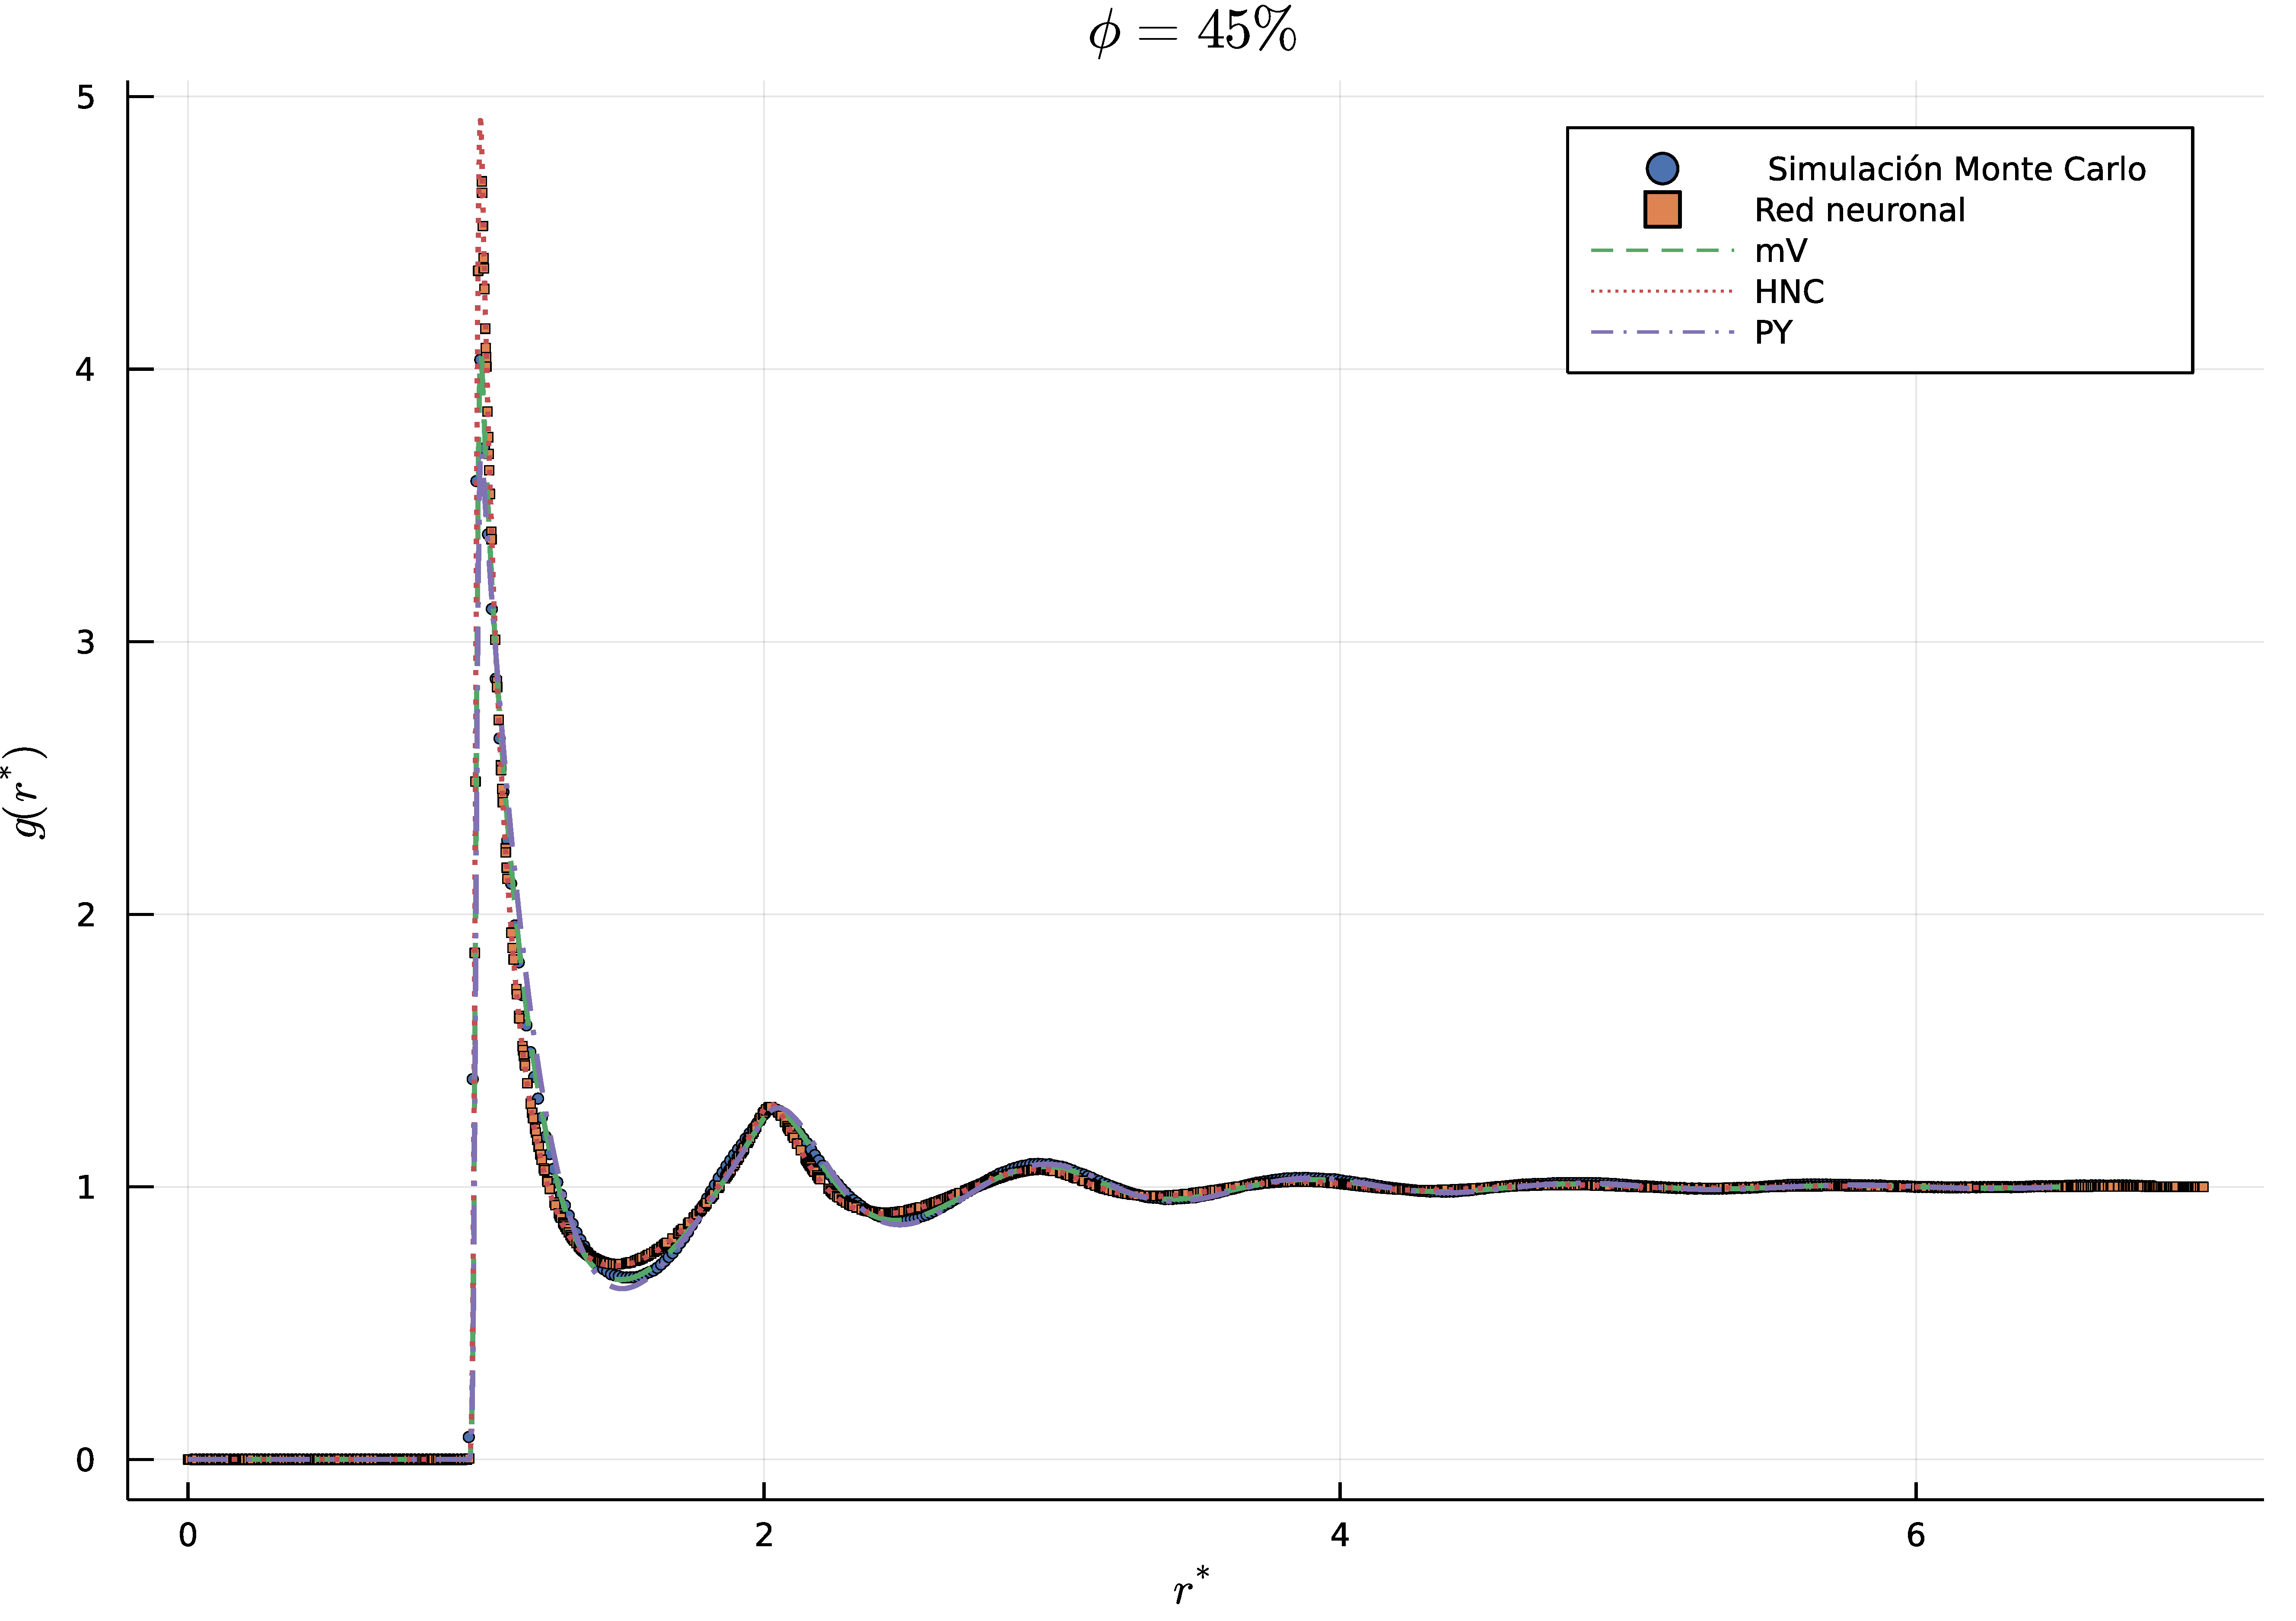
\includegraphics[width=0.47\textwidth]{figuras/capitulo-3/p=0.45.pdf} \\
        (c) & (d) \\[6pt]
    \end{tabular}
    \captionsetup{singlelinecheck=off}
    \caption[Funciones de distribución radial con redes neuronales.]{Funciones de distribución radial obtenidas con simulación por computadora y mediante el uso de la metodología descrita en este capítulo, usando redes neuronales. Se presentan cuatro densidades: 
    \begin{enumerate*}[label=(\alph*),itemjoin={,\enspace}]
        \item $\phi=\num{0.15}$
        \item $\phi=\num{0.25}$
        \item $\phi=\num{0.35}$
        \item $\phi=\num{0.45}$
    \end{enumerate*}
    . En cada una, se muestran las comparaciones con tres diferentes aproximaciones para la función puente: \emph{mV}, Verlet modificada; \emph{PY}, Percus-Yevick; y \emph{HNC}, Hypernetted Chain.
    }
    \label{fig:estructuras-neuronales}
\end{figure}

Con todos los elementos descritos en las secciones anteriores, los resultados obtenidos en 
esta sección se muestran en la figura~\ref{fig:estructuras-neuronales}, que corresponden
a las funciones de distribución radial, $g(r^*)$, de las densidades del líquido estudiadas.
Estas funciones describen la estructura del líquido, y son el tema central de estudio
de la metodología descrita en este capítulo.

\subsection{Densidades bajas}
Primero se analizarán y discutirán las densidades bajas $\phi=\numlist{0.15; 0.25}$,
las cuales corresponden a las gráficas (a) y (b) en la figura~\ref{fig:estructuras-neuronales}.
Los resultados que se observan es que, a densidades bajas, las aproximaciones HNC y
redes neuronales son más precisas que Percus-Yevick y Verlet modificada, sin embargo
ninguna de estas cuatro aproximaciones logra obtener resultados comparables a aquellos
de la simulación por computadora. En especial, es importante observar que
la aproximación de redes neuronales es un poco más precisa que la HNC, aunque sigue 
sobreestimando el pico principal que se encuentra en $r^* = \sigma$.
Por otro lado, las aproximaciones de Percus-Yevick y Verlet modificada subestiman el pico
principal para ambas densidades.

Tambíen es importante observar la forma funcional de $g(r^*)$. Para el caso de HNC y redes 
neuronales, parece ser que la forma es muy semejante entre ambas aproximaciones, e incluso 
pudiera ser la misma. Esto implica que, de alguna forma, los pesos de la red neuronal se 
ajustaron lo suficiente tal que la aproximación resulta ser HNC, o algo semejante.
Dicho de otra forma, los pesos son muy cercanos a cero tal que al ser
evaluada la red neuronal, la aproximación es muy semajante a HNC.
Otro factor importante a observar es que esta forma también es ligeramente diferente a
la encontrada con las simulaciones por computadora, pues las aproximaciones de
Percus-Yevick y Verlet modificada son más precisas en este aspecto.

\subsection{Densidades altas}
Ahora se discutirán los resultados para las densidades altas $\phi=\numlist{0.35; 0.45}$,
las cuales corresponden a las gráficas (c) y (d) en la figura~\ref{fig:estructuras-neuronales}.
De la misma forma que para las densidades bajas, las aproximaciones HNC y redes neuronales
para las densidades altas no son muy precisas. Ahora, y como era de esperarse, las 
aproximaciones Percus-Yevick y Verlet modificada son las más precisas, siendo Verlet
modificada la más precisa de todas. Esto se puede observar en la figura~\ref{fig:estructuras-neuronales}
al ver que el pico principal está muy bien estimado por la aproximación Verlet modificada,
mientras que las aproximaciones HNC y redes neuronales sobreestiman por mucho este valor.

Por otro lado, y semejante al caso para densidades bajas, la forma funcional de $g(r^*)$
es diferente entre la obtenida con simulación por computadora de aquella utilizando la
aproximación de redes neuronales. De hecho, al igual que antes, el resultado es muy
semejante al obtenido con la aproximación HNC. Esto es algo importante de observar, y
sustenta la hipótesis de que la aproximación de red neuronal se reduce a la aproximación
HNC.
Esto implica que la red neuronal en realidad está aproximando una función puente
$B(\vecr) \approx 0$.
Si se observan las aproximaciones de Percus-Yevick y Verlet modificada, volvemos a observar
que la aproximación de Verlet modificada es la más precisa, pues la forma funcional de
$g(r^*)$ es muy semejante a la obtenida con simulación por computadora.